\documentclass[a4paper, 12pt]{article}
\usepackage[portuges]{babel}
\usepackage[utf8]{inputenc}
\usepackage{amsmath}
\usepackage{indentfirst}
\usepackage{graphicx}
\usepackage{multicol,lipsum}
\usepackage{xcolor}
\usepackage{multicol}
\usepackage{listings}
% ---
% PACOTES
% ---

\usepackage{caption}
\usepackage{mathrsfs}
\DeclareCaptionType{equ}[][]
\usepackage{url}
\usepackage{lmodern}			% Usa a fonte Latin Modern
\usepackage[T1]{fontenc}		% Selecao de codigos de fonte.
\usepackage[utf8]{inputenc}		% Codificacao do documento (conversão automática dos acentos)
\usepackage{indentfirst}		% Indenta o primeiro parágrafo de cada seção.
\usepackage{amssymb}
\usepackage{color}				% Controle das cores
\usepackage{graphicx}			% Inclusão de gráficos

\usepackage{microtype} 			% para melhorias de justificação
\usepackage{chngcntr}
\usepackage{booktabs}
\usepackage{float} 				% Set posição da figura
\usepackage[bottom]{footmisc} 
\usepackage{subfig} 			% Inserir subfiguras
%\usepackage[table,xcdraw]{xcolor} 	% Cor de preenchimento das tabelas
\usepackage{multirow} 			%mesclar cel em tabelas
\usepackage{verbatim}			%Inserir codigos fontes e comentários em massa

\usepackage{lipsum}				% para geração de dummy text
\usepackage{amsmath}
\usepackage[bottom]{footmisc}
\usepackage{footnote}
%\usepackage{fnpos}
%\usepackage{ftnxtra}
%\usepackage{listings} 			%Inserir códigos fontes
\usepackage{rotating} 			%Rotação de páginas
\usepackage{placeins}			% Forçar o posicionamento da figura
\usepackage[top=3cm, bottom=2cm, left=3cm, right=2cm]{geometry}

\definecolor{vgreen}{RGB}{104,180,104}
\definecolor{vblue}{RGB}{49,49,255}
\definecolor{vorange}{RGB}{255,143,102}
\definecolor{mGreen}{rgb}{0,0.6,0}
\definecolor{mGray}{rgb}{0.5,0.5,0.5}
\definecolor{mPurple}{rgb}{0.58,0,0.82}
\definecolor{backgroundColour}{rgb}{0.95,0.95,0.92}

\lstdefinestyle{CStyle}{
    backgroundcolor=\color{backgroundColour},   
    commentstyle=\color{mGreen},
    keywordstyle=\color{magenta},
    numberstyle=\tiny\color{mGray},
    stringstyle=\color{mPurple},
    basicstyle=\footnotesize,
    breakatwhitespace=false,         
    breaklines=true,                 
    captionpos=b,                    
    keepspaces=true,                 
    numbers=left,                    
    numbersep=5pt,                  
    showspaces=false,                
    showstringspaces=false,
    showtabs=false,                  
    tabsize=2,
    frame=shadowbox,
    language=C
}

\usepackage[utf8]{inputenc}

% Default fixed font does not support bold face
\DeclareFixedFont{\ttb}{T1}{txtt}{bx}{n}{12} % for bold
\DeclareFixedFont{\ttm}{T1}{txtt}{m}{n}{12}  % for normal

% Custom colors
\usepackage{color}
\definecolor{deepblue}{rgb}{0,0,0.5}
\definecolor{deepred}{rgb}{0.6,0,0}
\definecolor{deepgreen}{rgb}{0,0.5,0}

\usepackage{listings}

% Python style for highlighting
\newcommand\pythonstyle{\lstset{
language=Python,
basicstyle=\ttm,
otherkeywords={self},             % Add keywords here
keywordstyle=\ttb\color{deepblue},
emph={MyClass,__init__},          % Custom highlighting
emphstyle=\ttb\color{deepred},    % Custom highlighting style
stringstyle=\color{deepgreen},
frame=tb,                         % Any extra options here
showstringspaces=false            % 
}}


% Python environment
\lstnewenvironment{python}[1][]
{
\pythonstyle
\lstset{#1}
}
{}

% Python for external files
\newcommand\pythonexternal[2][]{{
\pythonstyle
\lstinputlisting[#1]{#2}}}

% Python for inline
\newcommand\pythoninline[1]{{\pythonstyle\lstinline!#1!}}

\begin{document}
%\maketitle

\begin{titlepage}
	\begin{center}
	
	%\begin{figure}[!ht]
	%\centering
	%\includegraphics[width=2cm]{c:/ufba.jpg}
	%\end{figure}

		\Huge{Universidade Federal do Rio Grande do Norte}\\
		\large{Departamento de Engenharia de Computação e Automação}\\ 
		\
		\vspace{15pt}
        \vspace{95pt}
        \
        
		\LARGE{Lista 1 Redes Neurais.}
		%\title{{\large{Título}}}
		\vspace{3,5cm}
	\end{center}
	
	\begin{flushleft}
		\begin{tabbing}
			Alunos: Reinaldo Agostinho de Souza Filho, Paulo Victor Queiroz Correia\\
            Professor: Adrião Duarte Doria Melo \
	\end{tabbing}
 \end{flushleft}
	\vspace{1cm}
	
	\begin{center}
		\vspace{\fill}
			 Abril \\
		 2020
			\end{center}
\end{titlepage}
%%%%%%%%%%%%%%%%%%%%%%%%%%%%%%%%%%%%%%%%%%%%%%%%%%%%%%%%%%%

% % % % % % % % %FOLHA DE ROSTO % % % % % % % % % %

\begin{titlepage}
	\begin{center}
	
	%\begin{figure}[!ht]
	%\centering
	%\includegraphics[width=2cm]{c:/ufba.jpg}
	%\end{figure}

		\Huge{Universidade Federal do Rio Grande do Norte}\\
		\large{PROGRAMA DE PÓS-GRADUAÇÃO EM ENGENHARIA ELÉTRICA E DE COMPUTAÇÃO }\\ 
\vspace{15pt}
        
        \vspace{85pt}
        
		\textbf{\LARGE{Atividade avaliativa}}
		\title{\large{Lista de exercícios 1.}}
	%	\large{Modelo\\
     %   		Validação do modelo clássico}
			
	\end{center}
\vspace{1,5cm}
	
	\begin{flushright}

   \begin{list}{}{
      \setlength{\leftmargin}{4.5cm}
      \setlength{\rightmargin}{0cm}
      \setlength{\labelwidth}{0pt}
      \setlength{\labelsep}{\leftmargin}}

      \item \large{Lista de exercícios 1.}

      \begin{list}{}{
      \setlength{\leftmargin}{0cm}
      \setlength{\rightmargin}{0cm}
      \setlength{\labelwidth}{0pt}
      \setlength{\labelsep}{\leftmargin}}
      \

			\item Alunos: 
			    \subitem Reinaldo Agostinho de Souza Filho \
			    \subitem Paulo Victor Queiroz Correia 
            \item Professor: Adrião Duarte Doria Melo \

      \end{list}
   \end{list}
\end{flushright}
\vspace{1cm}
\begin{center}
		\vspace{\fill}
		 Abril\\
		 2020
			\end{center}
\end{titlepage}
\newpage
% % % % % % % % % % % % % % % % % % % % % % % % % %
\newpage
\tableofcontents


\section{Questão 1}

i)


$\phi (v) = \frac{1}{1+e^{-av}}$

$\phi' (v) = \frac{0(1+e^{-av})-(-ae^{-av})}{(1+e^{-av})^2}$

$\phi' (v) = \frac{ae^{-av}}{(1+e^{-av})^2}$

$a\phi(v) [1-\phi(v)] = a \frac{1}{1+e^{-av}}[1- \frac{1}{1+e^{-av}} ]$

$a\phi(v) [1-\phi(v)] = a \frac{1}{1+e^{-av}}[\frac{1+e^{-av}}{1+e^{-av}}- \frac{1}{1+e^{-av}} ]$

$a\phi(v) [1-\phi(v)]=\frac{a}{1+e^{-av}}\frac{e^{-av}}{1+e^{-av}}$

$a\phi(v) [1-\phi(v)]=\frac{ae^{-av}}{1+e^{-av}} = \phi'(v)$

\

ii)

$\phi(v) = tanh(\frac{av}{2})$

\

Pela definição da tangente hiperbólica e a regra da cadeia temos que 

\

$\phi'(v)=\frac{a}{2}sech^2(\frac{av}{2})$


$\phi'(v)=\frac{a}{2}[1-tanh^2(\frac{av}{2})]$

$\phi'(v)=\frac{a}{2}[1-\phi(v)^2])$

iii)

Utilizando o seguinte algoritmo utilizando a = 1 fiz o comparativo das funções de ativação.


\begin{lstlisting}[style=CStyle]
import matplotlib.pyplot as plt 
import numpy as np 
import math 
  
v = np.linspace(-10, 10, num=100) 
sig = 1/(1 + np.exp(-v)) 
tanh = np.arctan(v/2)
fig, ax = plt.subplots()

ax.plot(v, sig,'-b', label='sigmoid') 
ax.plot(v,tanh,'-r',label ='tangsigmoid')
ax.plot(v,np.maximum(0,v),'-g',label='Re-Lu')
leg = ax.legend()
plt.ylabel("Functions ") 
  
plt.show() 
\end{lstlisting}
\begin{figure}[H]
    \centering
    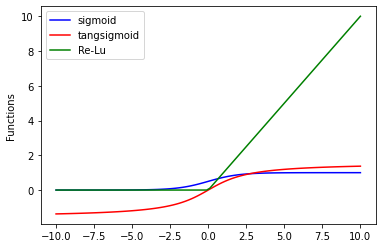
\includegraphics[width=10cm]{figuras/plots.png}
    \caption{Comparativo das funções de ativação.}
    \label{fig:plot1}
\end{figure}

iv)
Utilizando o seguinte algoritmo obtivemos o resultado:

\begin{lstlisting}[style=Cstyle]
x = np.linspace(-10,10,100)
w = np.array([-1])

w = np.append(w,np.random.rand(99))

v=w.transpose()@x


def dsig(v):
  return a*np.exp(-a*v)/(1 + np.exp(-a*v))
def dtanh(v):
  return (a/2)*(1-np.arctan(a*v/2)**2)
def drelu(v):
    return np.multiply(v>=0,1)

print("para um neuronios")
print("derivada da sigmoid: ",dsig(v))
print("derivada da tansigmoid: ",dtanh(v))
print("derivada da relu(degrau): ",drelu(v))

print("para dois neuronios")
w = np.random.rand(100,2)
v = w.transpose()@x
print("derivada da sigmoid: ",dsig(v))
print("derivada da tansigmoid: ",dtanh(v))
print("derivada da relu(degrau): ",drelu(v))


\end{lstlisting}

Obtendo a seguinte saída:

\begin{lstlisting}
para um neuronios
derivada da sigmoid:  1.9999915552473924
derivada da tansigmoid:  -0.9896993190121113
derivada da relu(degrau):  0
para dois neuronios
derivada da sigmoid:  [0.06193825 1.99932349]
derivada da tansigmoid:  [-0.09116056 -0.75711874]
derivada da relu(degrau):  [1 0]
\end{lstlisting}

\section{Questão 2}

\subsection{Distância Euclidiana}

A distância Euclidiana é a métrica simplesmente é a distância geométrica no espaço multidimensional.
Ela é calculada como: \\

$d(\Vec{x},\Vec{y})=\sqrt{\sum_{i=1}^p (x_i-y_i)^2} $

\subsection{Distância Mahalanobis}
Essa métrica indica a dissimilaridade entre dois vetores aleatórios, também é conhecido 
distância estatística por isso, dados dois vetores aleatórios $\Vec{x},\Vec{y}$ com mesma 
distribuição e com matriz covariância S:\\


$d(\Vec{x},\Vec{y})=\sqrt{(\Vec{x}-\Vec{y})'S^{-1}(\Vec{x}-\Vec{y})} = \sqrt{\frac{(x_1-y_1)^2}{s_1^2}+...+\frac{(x_p-y_p)^2}{s_p^2}} $

\subsection{Métrica de Minkowski}

Utilizada da geometria da relatividade a métrica de Minkowski calcula a 
raiz da distância absoluta dentre dois tensores descrito analiticamente abaixo de forma 
semelhante a distância euclidiana\\

$d(\Vec{x},\Vec{y})=n\sqrt{\sum_{i=1}^p |x_i-y_i|^n} $

\subsection{Coeficiente de Correlação de Pearson}

Esse coeficiente indica o grau de correlação entre douas variáveis na escala métrica, assumindo valores entre -1 e 1\\

$\rho = \frac{\sum_Pi=1^n(x_i-\Bar{x})(y_i-\Bar{y})}{\sqrt{\sum_{i=1}^n(x_i-\Bar{x})^2}\sqrt{\sum_{i=1}^n(y_i-\Bar{y})^2}}
=\frac{cov(X,Y)}{\sqrt{var(X).var(Y)}}$

\subsection{Similaridade Cosseno}

Essa métrica indica a distância angular entre dois pontos a partir da origem.\\

$cos(x,y)=\frac{\sum_i=1^n x_k y_k }{\sqrt{\sum_i=1^n x_k^2}{\sqrt{\sum_i=1^n y_k^2}}} $ \\

Se a similaridade for 1 o angulo é de 0 ou $\pi$ se for 0 o ângulo é $\frac{\pi}{2} ou - \frac{\pi}{2}$


\section{Questão 3}

a)\\

$H(n)=H(n-1)+g(n)g(n)^t $ \\

$H(n-1) = \sum_{k=1}^{n-1} g(k)g(k)^t$

$H(n) = \sum_{k=1}^{n} g(k)g(k)^t$

$H(n-1) =[ \sum_{k=1}^{n} g(k)g(k)^t] - g(n)g(n)^t$

$H(n-1) = H(n) - g(n)g(n)^t$

$H(n)=H(n-1)+g(n)g(n)^t $ \\

b)\\

Dados: $A=H(n) B^{-1} = H(n-1) C=g(n) D=1 $\\

Substituindo a primeira equação temos o que foi provado na questão anterior que:

$H(n)=H(n-1)+g(n)1g(n)^t $

aplicando o o lema da inversão matricial teremos:\\

$H(n)^{-1} = H(n-1)^{-1} - H(n-1)^{-1} g(n) (1+g(n)^t H(n-1)^{-1}g(n))^{-1}g(n)^t H(n-1)^{-1}$\\

$H(n)^{-1} = H(n-1)^{-1} - \frac{H(n-1)^{-1} g(n)g(n)^t H(n-1)^{-1}}{1+g(n)^t H(n-1)^{-1}g(n)}$

\section{Questão 4}

Tomando que dado um $f(x)=0$ temos que $f(x)f(x)=0$ logo $f(z)^2 = 0$ sendo então o conjunto de pontos z pontos de mínimos absolutos de x se existir solução para f(x)=0
\\
Seja A uma matriz simétrica e definida positiva, e consideremos uma forma quadrática auxiliar:

$f(x)= \frac{x^T Ax}{2} -b^T x + c$

que transforma vetores em números reais. Como a forma é quadrática há apenas um vetor que minimiza f e é exactamente o ponto crítico, solução de

$\nabla f(x) = 0, \nabla f(x)=\frac{(A^T +A)x}{2}-b = Ax+b$

Assim, se encontrarmos o ponto de mínimo, ele será solução do sistema linear Ax = b.

Consideramos métodos iterativos de optimização do tipo:

$x^{(n+1)}=x^{(n)}+a_nr^{(n)}$


onde r é o vetor que indica a direção da desicida.


a) Método do gradiente conjugado:
Teorema: Um método de direcções conjugadas atinge a solução ao fim de N iterações.

considerando $e^{(n)}=x-x^{(n)}$ o erro do x encontrado na n-ésima iteração
 
considerando sabido o método dos gradientes apresentamos-lo como:\\

$r^{(i)} = b- Ax^{(i)} $\\

$\lambda^{(i)}=\frac{r^{(0)T} r^{(0)} } {r^{(0)T}Ar^{(0)}}$\\

$x^{(i+1)}=x^{(i)}+\lambda^{(i)}r^{(n)}$    

Porém em muitos casos várias vezes pode-se tomar uma mesma direção $r^{(i)}$ nomaremos então um conjunto de direções conjugadas {$d_0,d_1,...,d_{n-1}$} em até n iterações.

lembrando que dois vetores x e y serão conjugados se:
\\

$x^TAy=y^TAx=0$\\

Dado um $x^{(0)},$ faremos $d^0=r^0=b-Ax$ e x(1) pela equação:

$x^{(1)}=x^{(0)}+\lambda^{(0)}d^{(0)}$

o tamanho do passo é feito extraindo a derivada com relação a lambda de $x^{(i)}$

$\frac{df(x^{(1)})}{d\lambda} = -r^{(1)T}d^{(0)} $

para que $r^{(1)}=r^{(0)}-\lambda^{(0)}Ad^{(0)}$ seja ortogonal à direção $d^{(1)} = r^{(1)}+\beta^{(1)}d^{(0)}$ precisaremos adequar a escolha de $\beta$\\

assim como: $r^{(1)T}d^{(1)}=0$\\

$r^{(0)}- (\frac{r^{(0)T}r^{(0)}}{r^{(0)T}Ar^{(0)}}Ad^{(0)})^T (r^{(1)}+\beta^{(1)}d^{(0)})=0$\\

Simplificando temos:

$\beta^{(1)} = -\frac{d^{(0)T}Ar^{(1)}}{d^{(0)T}Ad^{(0)}} = -\frac{r^{(1)T}Ad^{(0)}}{d^{(0)T}Ad^{(0)}}$




\section{Questão 5}

Nesta questão, é necessário, inicialmente, gerarmos os dados de entrada e saídas correspondentes, em que a entrada do modelo será um conjunto de 3 bits que serão decodificados numa saída equivalente aos seus valores convertidos de binário para decimal, no intervalo de 0 até 7. Em seguida, serão adicionados um ruído branco em cada um desses bits, no intuito de atender aos critérios exigidos na questão.

O conjunto de entrada foi criado da seguinte maneira, como visto nas figuras \ref{fig:quest5_entrada1} e \ref{fig:quest5_entrada2}, em que é possível notar uma \textit{seed} fixa para tornar o experimento reproduzível, uma média constante de 0 para o ruído branco com desvio padrão de 0,4, e a partir daí foram gerados 1024 pontos binários aleatórios em cada entrada para serem usados no modelo de aprendizagem. Após esses pontos e o ruído branco serem gerados, somamos os 2 para obter um sinal de entrada ruidoso com a decodificação obtida pelos pontos sem ruído. 

\begin{figure}[h]
	\centering
 	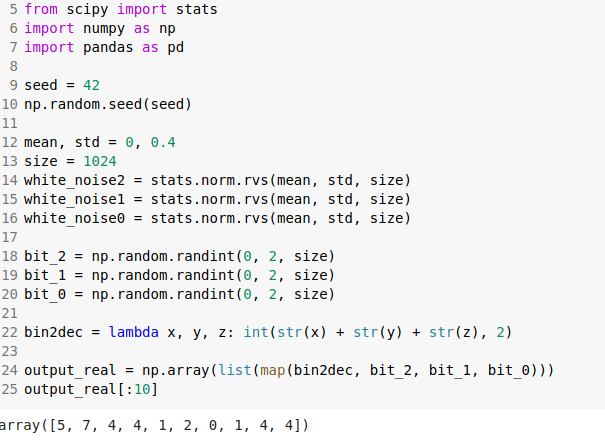
\includegraphics[width=0.7\linewidth]{figuras/quest5_entrada1.png}
    \caption{Gerando dados de entrada e saída para o modelo, com o mapeamento dos valores de entrada com suas respectivas saidas}
    \label{fig:quest5_entrada1}
\end{figure}
\FloatBarrier

\begin{figure}[h]
	\centering
 	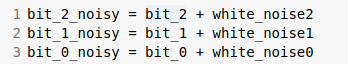
\includegraphics[width=0.6\linewidth]{figuras/quest5_entrada2.png}
    \caption{Somando bits de entrada ao ruído branco.}
    \label{fig:quest5_entrada2}
\end{figure}
\FloatBarrier
Para a geração de modelos de aprendizagem de máquina nesta lista, foi utilizado o pacote \textit{scikit-learn} em conjunto com os pacotes \textit{numpy}, \textit{scipy.stats} e \textit{pandas}.

Nesta questão, para implemntarmos uma rede ADALINE que implementasse o algoritmo Least Mean Square (LMS), utilizamos o modelo classificador \textit{SGDClassifier} para realizar isto, o qual utilizará a estratégia de um contra todos para decodificar os bits ruidosos. Além disso, será realizado o ajuste dos hiperparâmetros do modelo, com a intenção de buscar o modelo com os parâmetros com a melhor acurácia de validação obtidos no treinamento, e então usar esse modelo para classificar as entradas do conjunto de testes, que representa 25\% dos conjunto de dados.

\begin{figure}[h]
	\centering
 	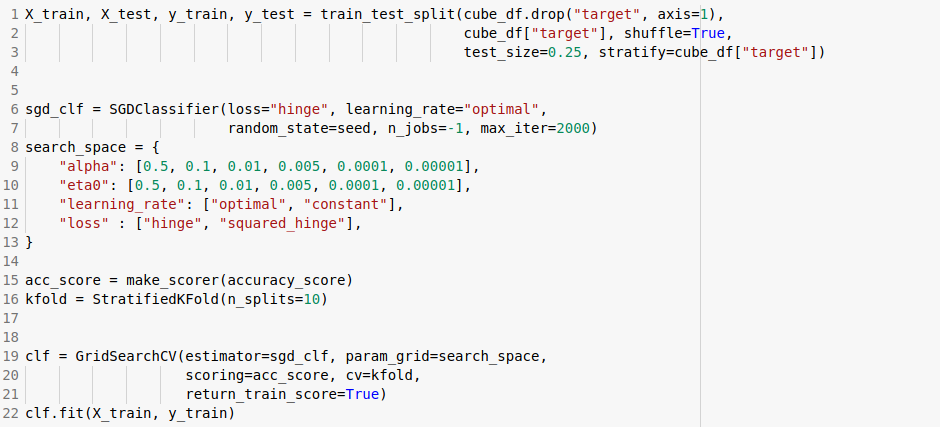
\includegraphics[width=\linewidth]{figuras/quest5_model1.png}
    \caption{Definição do modelo, do espaço de busca dos parâmetros ótimos e realização do treinamento a partir da validação cruzada de 10 divisões.}
    \label{fig:quest5_modelo}
\end{figure}
\FloatBarrier

A partir do treinamento, foi obtido um modelo ótimo dentro do espaço de busca, o qual possuia a melhor média de acurácia, e a partir desse modelo com os parâmetros da figura \ref{fig:quest5_parametros}, verificamos que o a acurácia no conjunto de treinamento é de 67,97\%.

\begin{figure}[h]
	\centering
 	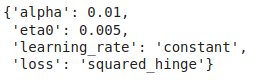
\includegraphics[width=0.6\linewidth]{figuras/quest5_parametros.png}
    \caption{Parâmetros ótimos selecionados na busca.}
    \label{fig:quest5_parametros}
\end{figure}
\FloatBarrier

\section{Questão 6}

Inicialmente, temos uma fonte de sinal discreto a partir da equação definido por: \begin{equation}
s(n) = sen(0,075n\pi)
\end{equation}Um sensor capta esse sinal e o reproduz digitalmente da seguinte forma:
\begin{equation}
x(n) = s(n) + v_1(n)
\end{equation}
Em que $v_1(n)$ é o ruído captado pelo sensor 1 somado a um ruído branco com média 0 e desvio padrão 1, definido por: 
\begin{equation}\label{v1}
v_1(n) = -0,5v_1(n-1) + v(n)
\end{equation}Da mesma forma, o sensor 2 capta uma fonte de ruído indesejado da seguinte forma:
\begin{equation}\label{v2}
v_2(n) = 0,8v_2(n-1)+v(n)
\end{equation}
Para a resolução, definimos um ruído branco chamado \textit{white\_noise} e criamos uma amostragem atrasada desse ruído e finalmente geramos os sinas de $v_1(n)$ e $v_2(n)$ a partir das equações \ref{v1} e \ref{v2}.

Para a criação de um perceptron puramente linear o qual implementa o algoritmo \textit{LMS}, utilizamos o modelo \textit{SGDRegressor} do pacote \textit{scikit-learn}, pois ele implementa o algoritmo em questão. Os dados de entrada foram gerados no espaço linear de 0 a 100 com 5000 amostras equidistantes e embaralhados para o treinamento.

A métrica para avaliar o treinamento foi a \textit{Root Mean Squared Error}(RMSE) e o processo de treinamento e geração do gráfico para podermos visualizar a performance do modelo graficamente pode ser visto na imagem \ref{fig:quest6_code}.

\begin{figure}[h]
	\centering
 	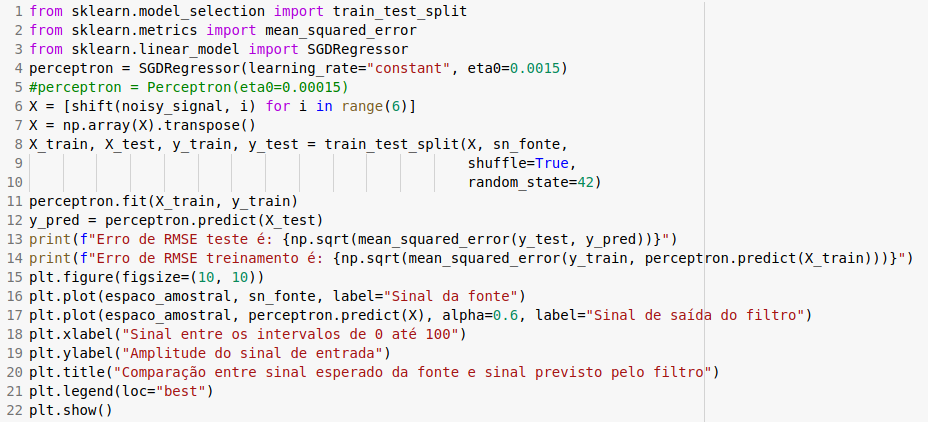
\includegraphics[width=0.8\linewidth]{figuras/quest6_code.png}
    \caption{Código usado para o treinamento do modelo e geração das métricas e gráficos para análise de desempenho.}
    \label{fig:quest6_code}
\end{figure}
\FloatBarrier

Em que separamos o conjunto de dados em 75\% para treinamento do modelo e 25\% para teste, e os resultados podem ser vistos a seguir na figura \ref{fig:quest6_saida}.

\begin{figure}[h]
	\centering
 	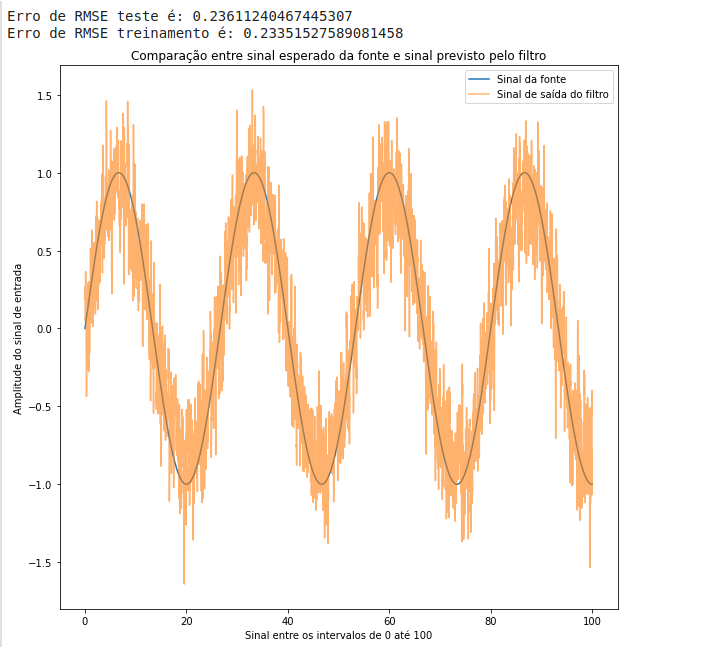
\includegraphics[width=0.8\linewidth]{figuras/quest6_saida.png}
    \caption{Métricas de desempenho para os dados de treinamento e gráfico comparativo do sinal original e o previsto pelo modelo.}
    \label{fig:quest6_saida}
\end{figure}
\FloatBarrier

A partir desses resultados, podemos observar que o algoritmo conseguiu regredir aproximadamente bem, com boas métricas de treinamento e teste (0,2335 e 0,2361 respectivamente), não evidenciando que houve \textit{overfitting} ou \textit{underfitting} do modelo a partir do conjunto de dados.

\section{Questão 7}

O algoritmo de retropropagação é amplamente utilizado como forma de atualizar os pesos em uma rede neural do tipo \textit{feedforward}, possuindo dois tipos de atualização: \textit{online} e por lote. Nesta questão, deduziremos como se dá a atualização de pesos com esse algoritmo no modo de treinamento por lote e uma revisão bibliográfica de alguns materiais sobre como paraleliza-lo.

Inicialmente, é necessário definir as equações de função de custo instantâneo e função de custo médio, apresentadas nas equações \ref{eq:quest7_custo_inst} e \ref{eq:quest7_custo_medio}.

\begin{equation}\label{eq:quest7_custo_inst}
    E(n) = \frac{1}{2} \sum\limits_{j\epsilon C} e^2_j(n)
\end{equation}

\begin{equation}
    E_{med} = \frac{1}{N} \sum\limits_{n=1}^{N} E(n) =  \frac{1}{2N}\sum\limits_{n=1}^{N}\sum\limits_{j\epsilon C} e^2_j(n)
\end{equation}

Em que $C$ é o conjunto de todos os neurônios da camada de saída da rede, $N$ é o número total de dados que serão usados no treinamento, $E$ é a função custo do modelo e $e_j$ é o erro de saída de um elemento do conjunto de treinamento.

Em seguida definimos a regra delta, que será usada para atualizar os pesos com a função de custo médio, visto que estamos analisando a retropropagação por lote.

\begin{equation}\label{eq:quest7_regradelta}
    \Delta w_{ji} = -\eta \frac{\partial E_{med}}{\partial w_{ji}}
    =-\frac{\eta}{N} \sum\limits_{n=1}^{N} e_j(n) \frac{\partial e_j(n)}{\partial w_{ji}}
\end{equation}

Para prosseguirmos, a derivada de $\frac{\partial e_j(n)}{\partial w_{ji}}$, precisamos a regra da cadeia da seguinte forma:

\begin{equation}
    \frac{\partial e_j(n)}{\partial w_{ji}} = \frac{\partial e_j(n)}{\partial y_j(n)}
                                              \frac{\partial y_j(n)}{\partial v_j(n)}
                                              \frac{\partial v_j(n)}{\partial w_{ji}}
\end{equation}

Como $e_j(n) = d_j(n) - y_j(n)$, $\frac{\partial e_j(n)}{\partial y_j(n)} = -1$.

Assim como $y_j(n) = \varphi_j (v_j(n))$, $\frac{\partial y_j(n)}{\partial v_j(n)}=\varphi_j' (v_j(n))$, em que $\varphi_j(.)$ é a função de ativação do neurônio em questão.

Finalmente, como $v_j(n) = \sum\limits_{i=0}^m w_{ji}(n)y_i(n)$, podemos concluir que $\frac{\partial v_j(n)}{\partial w_{ji}} = y_i(n)$

Juntando tudo, temos: 

\begin{equation}
   \frac{\partial e_j(n)}{\partial w_{ji}} = -
                                             \varphi_j' (v_j(n))
                                             y_i(n)
\end{equation}

Logo, considerando a equação de $\Delta w_{ji}$ para a atualização de cada peso $j$ a partir da retropropagação de erros dos neurônios a frente $i$, temos que o algoritmo de atualização por retropropagação por lote será o seguinte:

\begin{equation}
    \Delta w_{ji} = -\frac{\eta}{N} \sum\limits_{n=1}^{N} e_j(n)(-\varphi_j' (v_j(n))y_i(n))
                  = \frac{\eta}{N} \sum\limits_{n=1}^{N} e_j(n)\varphi_j' (v_j(n))y_i(n)
\end{equation}

Em que esta fórmula será aplicada a cada época durante o processo de treinamento.

Para a paralelização do algoritmo em questão, há diversos autores trabalhando na questão. (NOVOKHODKO, 2001)\cite{novokhodko2001parallel} utiliza a paralelização de rotinas de multiplicação de matrizes no MATLAB, através de métodos de \textit{message passing interface}. 

(FOOL, 1997)\cite{foo1997parallel} utiliza de duas técnicas para paraleliza-lo, nas quais os autores dividem o conjunto de treinamento em mais de um processador, por meio do paralelismo do conjunto de treinamento, e também utiliza alocações baseadas em programação de inteiros misturados, e comparando com um \textit{benchmark}, demonstra que a técnica reduz o tempo de treinamento por época do algoritmo.

Finalmente, (GHOLAMI, 2018)\cite{gholami2018integrated} explora a paralelização por lote e por domínio para o treinamento de redes de aprendizagem profundas, utilizando um solucionador do gradiente estocástico descendente (SGD) por mini-lotes, cujo objetivo é achar uma estratégia de paralelização eficiente para um lote de tamanho fixo utilizando P processos, utilizando um algoritmo de paralelização baeado em matrizes. 

\section{Questão 8}

\subsection{Item a}
A função para aproximar neste item é a função lógica:
\begin{equation}
f(x_1, x_2, x_3) = x_1 \oplus x_2 \oplus x_3
\end{equation}

Para o conjunto de treinamento, foi construida uma tabela da verdade com os resultados possíveis da equação lógica em questão, com um total de 8 linhas a serem utilizadas. O modelo de classificação utilizado é uma rede neural \textit{MLPClassifier} do pacote \textit{scikit-learn}, em que realizamos uma busca pelos hiperparâmetros ótimos do modelo utilizando o \textit{GridSearchCV}. A métrica de avaliação é a acurácia do modelo em questão. O treinamento pode ser visto a seguir na figura \ref{fig:quest8a_code}.

\begin{figure}[h]
	\centering
 	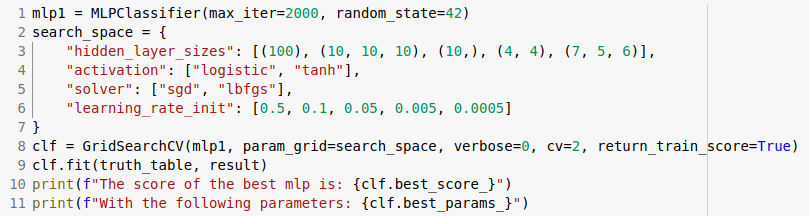
\includegraphics[width=0.9\linewidth]{figuras/quest8a_code.png}
    \caption{Código para a realização do treinamento no item a da questão 8.}
    \label{fig:quest8a_code}
\end{figure}
\FloatBarrier

Cujo resultado da acurácia para todo modelo foi de 0.625 e os parâmetros ótimos do modelo foram: 

With the following parameters: {'activation': 'tanh', 'hidden\_layer\_sizes': 100, 'learning\_rate\_init': 0.0005, 'solver': 'sgd'}.

\subsection{Item b}

Para este item, aproximar a função real:
\begin{equation}\label{eq:quest8b_function}
f(x_1, x_2) = \left(\frac{cos(2\pi x_1)}{1-(4x_1)^2} \frac{sen(\pi x_1)}{\pi x_1} \right)\left(\frac{cos(2\pi x_2)}{1-(4x_2)^2} \frac{sen(\pi x_2)}{\pi x_2}\right), -4\pi \leq x_1, x_2 \leq 4\pi
\end{equation}

Em que, dentro do intervalo definido, foram geradas 1000 amostras aleatórias uniformemente distribuídas. Da mesma forma que no item \textbf{a}, o treinamento foi feito buscado um modelo ótimo de redes neurais artificias voltados para regressão, com \textit{MLPRegressor}, como pode ser visto na figura \ref{fig:quest8b_train}.

\begin{figure}[h]
	\centering
 	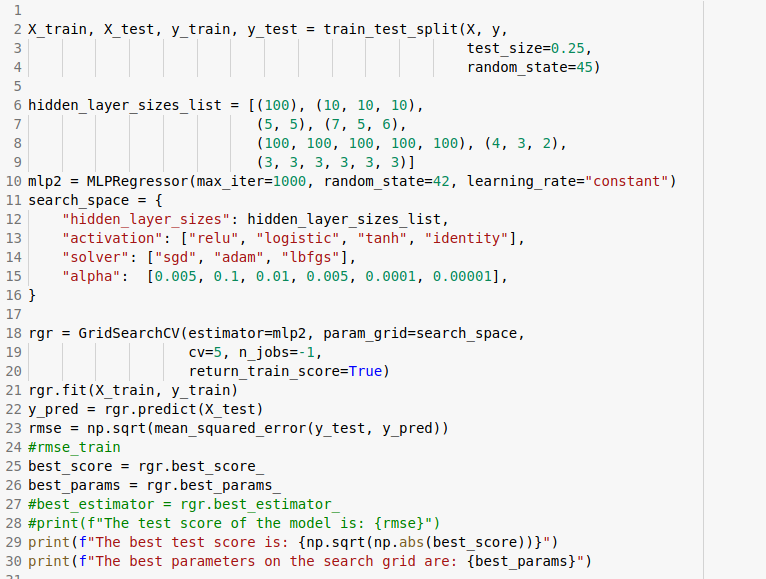
\includegraphics[width=0.9\linewidth]{figuras/quest8b_train.png}
    \caption{Código para a realização do treinamento no item a da questão 8.}
    \label{fig:quest8b_train}
\end{figure}
\FloatBarrier

Em que a média de performance do treinamento é de 0,1240 e de teste é de 16,90 na métrica RMSE, e observando esses resultados, podemos observar que é bem provável que ocorreu \textit{overfitting} no modelo de regressão, pois a diferença entre os valores das métricas no teste e no treinamento é bastante alta, se comparármos os dois valores. O gráfico comparando a curva de treinamento com a de validação pode ser visto na figura \ref{fig:quest8b_curva}.

\begin{figure}[h]
	\centering
 	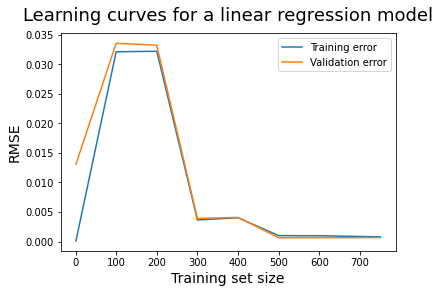
\includegraphics[width=0.5\linewidth]{figuras/quest8b_curve.png}
    \caption{Código para a realização do treinamento no item a da questão 8.}
    \label{fig:quest8b_curva}
\end{figure}
\FloatBarrier

\subsection{Item C}

Neste item, aproximamos a seguinte equação:

\begin{equation}
    f(\textbf{x}) = \frac{1}{2\pi |C|^{-1/2}}\sum\limits_{i=1}^{3} exp\left( -\frac{1}{2}  (x - m_i) ^t C^{-1} (x-m_i)\right) 
\end{equation}
Com $m_1= \begin{pmatrix} 0 \\ 0 \end{pmatrix}$,  $m_2= \begin{pmatrix} 0,5 \\ 0,5 \end{pmatrix}$, $m_2= \begin{pmatrix} -0,5 \\ -0,5 \end{pmatrix}$ e $C= \begin{pmatrix} 1 & 0 \\ 0 & 1 \end{pmatrix}$.

Em que o conjunto de treinamento foram 2 vetores com 1000 amostras com valores equidistantes entre -5 e 5, e o treinamento foi feito como no código da figura \ref{fig:quest8c_code}.

\begin{figure}[h]
	\centering
 	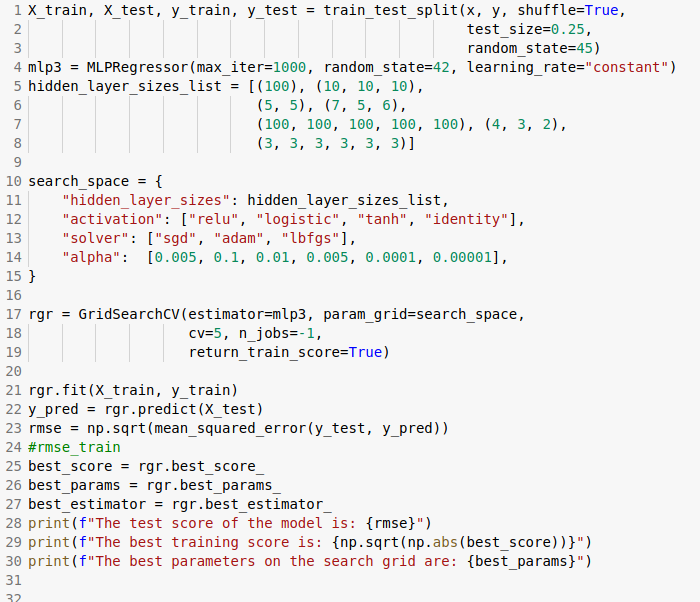
\includegraphics[width=0.6\linewidth]{figuras/quest8c_codigo.png}
    \caption{Código para a realização do treinamento no item c da questão 8.}
    \label{fig:quest8c_code}
\end{figure}
\FloatBarrier

Em que obtivemos o valor do \textit{RMSE} de teste de 0,153106 e de treinamento de 0,152956, sendo valores muito próximos, logo a chance do modelo apresentar problemas de \textit{overfitting} e \textit{underfitting} são muito baixas. Além disso, a busca forneceu os seguintes hiperparâmetros na busca em grade do treinamento:  'activation': 'tanh', 'alpha': 1e-05, 'hidden\_layer\_sizes': (3, 3, 3, 3, 3, 3), 'solver': 'sgd'.

Finalmente, a curva das métricas de treinamento x validação pode ser vista a seguir:
\begin{figure}[h]
	\centering
 	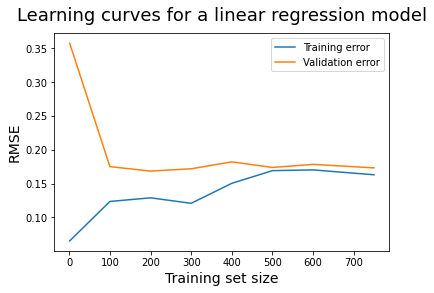
\includegraphics[width=0.5\linewidth]{figuras/quest8c_curva.png}
    \caption{Curva de treinamento e teste do modelo do item C.}
    \label{fig:quest8c_curva}
\end{figure}
\FloatBarrier


\section{Questão 9}

A função que desejamos aproximar é dada pela seguinte fórmula:

\begin{equation}\label{eq:quest9}
f(n) = 1+cos(1+cos^2(n))
\end{equation}


E o desenho da função pode ser vista na figura \ref{fig:quest9_original_plot}.

\begin{figure}[h]
	\centering
	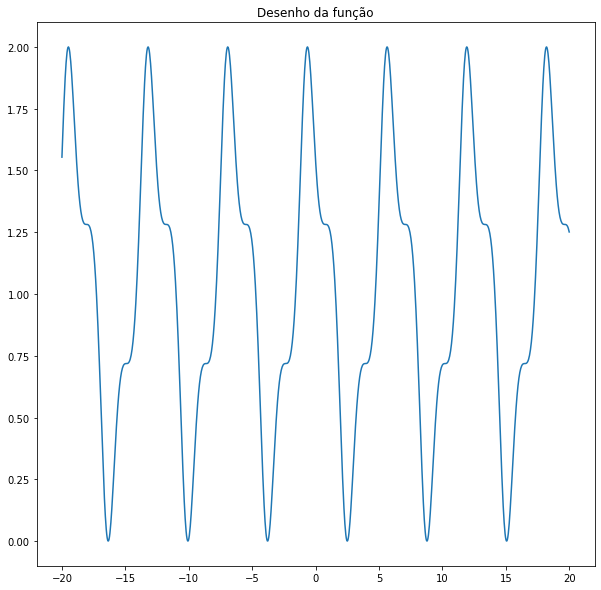
\includegraphics[width=0.7\linewidth]{figuras/quest9_original_plot}
    \caption{Plot da função \ref{eq:quest9}}
    \label{fig:quest9_original_plot}
\end{figure}
\FloatBarrier

Temos que o conjunto de dados da série temporal fica entre -20 e 20.

Após a geração do modelo, semelhante ao que foi feito na questão 5, o único parâmetro a ser ajustado será o número de atrasos que será utilizado no modelo de predição, começando de 1 até 3, e podemos ver que o treinamento foi feito como no código \ref{fig:quest9_train}, em que podemos verificar que a métrica de avaliação do modelo é a \textit{Root Mean Squared Error}.

\begin{figure}[h]
	\centering
	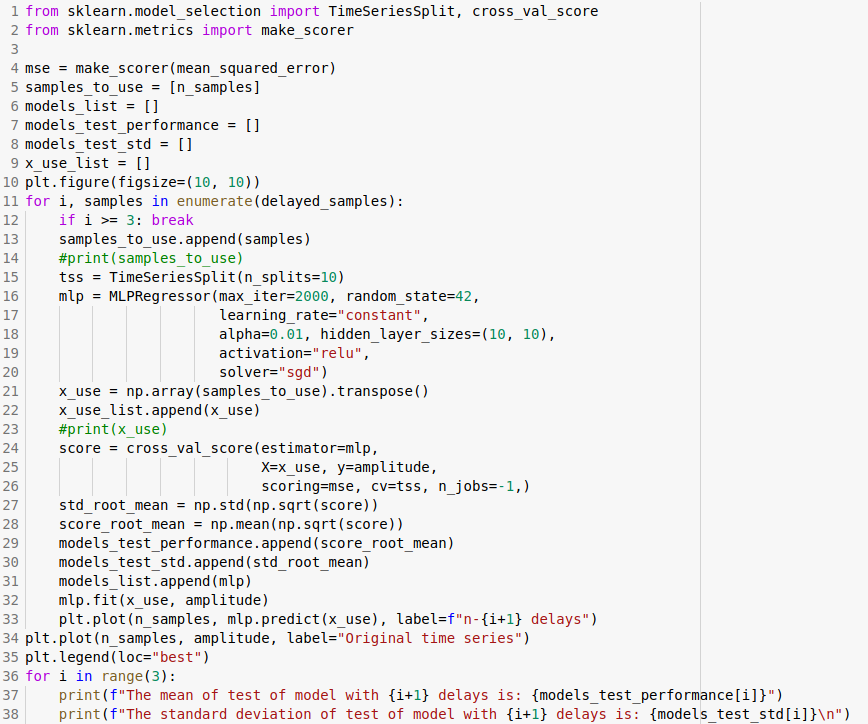
\includegraphics[width=0.85\linewidth]{figuras/quest9_train}
    \caption{Código utilizado para treinar os vários modelos de treinamento da questão.}
    \label{fig:quest9_train}
\end{figure}
\FloatBarrier

Como resultado, termos o seguinte:

\begin{figure}[h]
	\centering
	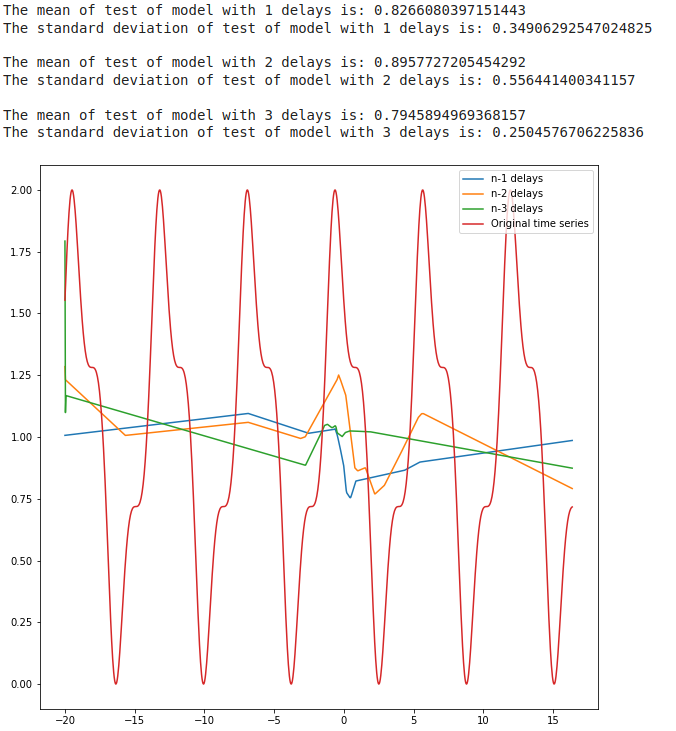
\includegraphics[width=0.8\linewidth]{figuras/quest9_saida}
    \caption{Funções aproximadas a partir do modelo de aprendizagem de máquina com atrasos de 0, 1, 2 e 3.}
    \label{fig:quest9_saida}
\end{figure}
\FloatBarrier
Em que podemos notar que mesmo utilizando mais de um atraso e vendo que os resultados apresentavam baixos valores nas métricas, o modelo de redes neurais não conseguiu aproximar bem a função de série temporal apresentada no enunciado.



\section{Questão 10}

Neste problema, é necessário comparar o desempenho de uma rede neural e uma máquina de vetor de suporte para classificarmos dois padrões dentro de um quadrado, como consta na figura \ref{fig:quest10_classes}, em que foi gerado pontos aleatórios seguindo o padrão proposto na questão.

\begin{figure}[h]
	\centering
	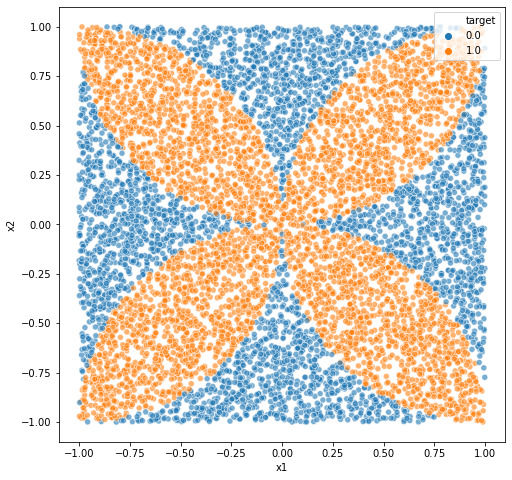
\includegraphics[width=0.8\linewidth]{figuras/quest10_classes.png}
    \caption{Gráfico com as classes a serem usadas nos modelos preditivos.}
    \label{fig:quest10_classes}
\end{figure}
\FloatBarrier

Para classificar o modelo, foi utilizado o conceito de \textit{Pipeline} somado ao que vinhamos fazendo com a busca pelos hiperparâmetros do modelo de predição, em que o \textit{Pipeline} entra para podermos testar mais de um algoritmo de aprendizagem de máquina, reduzir erros e o tempo para treinarmos as duas máquinas.

O treinamento foi feito a partir do código na figura \ref{fig:quest10_code}, em que separamos um conjunto de teste e treinamento de 25\% para teste e o restante para o treinamento do modelo, e geramos 8192 pontos aleatórios ao total.


\begin{figure}[h]
	\centering
	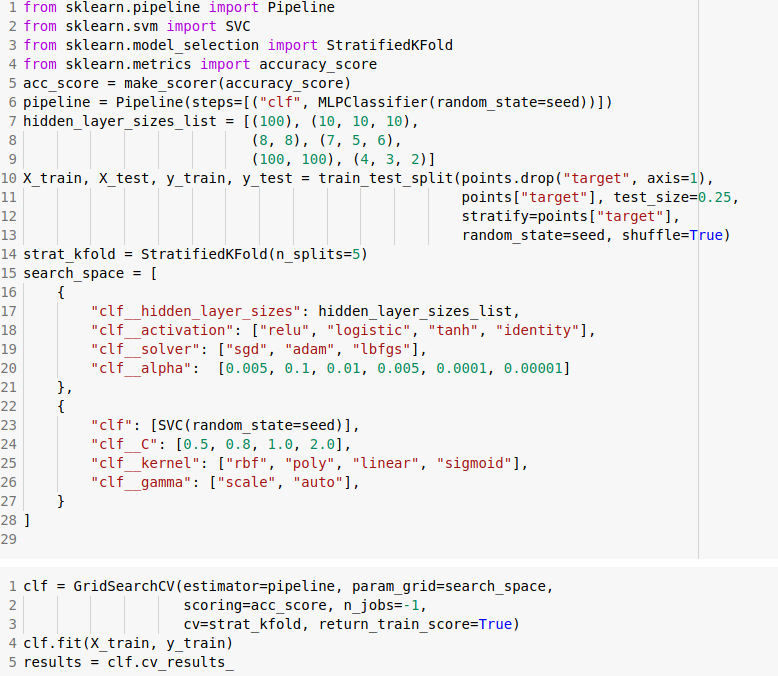
\includegraphics[width=0.8\linewidth]{figuras/quest10_code.png}
    \caption{Código usado para treinar os modelos de \textit{MLP} e \textit{SVM}.}
    \label{fig:quest10_code}
\end{figure}
\FloatBarrier

Como resultados, obtemos as seguintes métricas para o modelo de redes neurais e de vetor de suporte:


\begin{figure}[h]
	\centering
	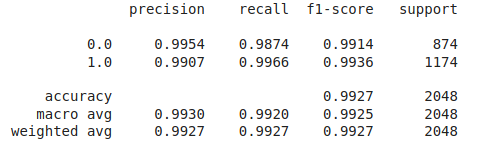
\includegraphics[width=0.5\linewidth]{figuras/quest10_summaryRNA.png}
    \caption{Sumário do desempenho para as redes neurais.}
    \label{fig:quest10_summaryRNA}
\end{figure}
\FloatBarrier

\begin{figure}[h]
	\centering
	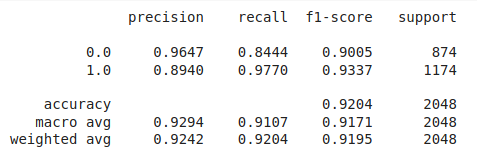
\includegraphics[width=0.5\linewidth]{figuras/quest10_summarySVM.png}
    \caption{Sumário do desempenho para a máquina de vetor de suporte.}
    \label{fig:quest10_summarySVM}
\end{figure}
\FloatBarrier

Em que podemos observar que o desempenho das redes neurais com o conjunto de teste foi superior ao da máquina de vetor de suporte, possuindo tanto acurácia quanto precisão e \textit{recall} superiores.

A matriz de confusão dos modelos pode ser vista a seguir em forma de mapa de calor, tanto para o modelo com redes neurais quanto para o modelo de \textit{SVM}.


\begin{figure}[h]
	\centering
	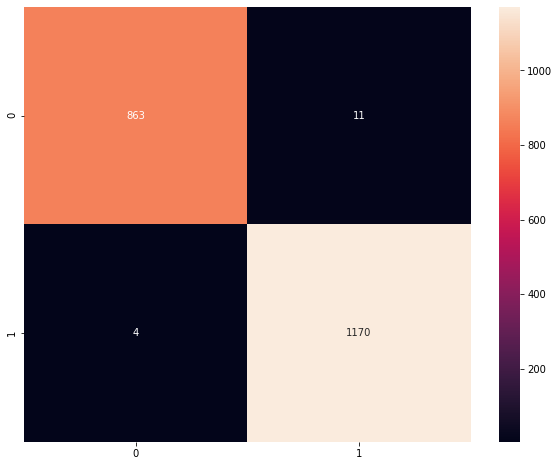
\includegraphics[width=0.5\linewidth]{figuras/quest10_confusaoRNA.png}
    \caption{Matriz de confusão no conjunto de dados de teste para a RNA.}
    \label{fig:quest10_confusaoRNA}
\end{figure}
\FloatBarrier



\begin{figure}[h]
	\centering
	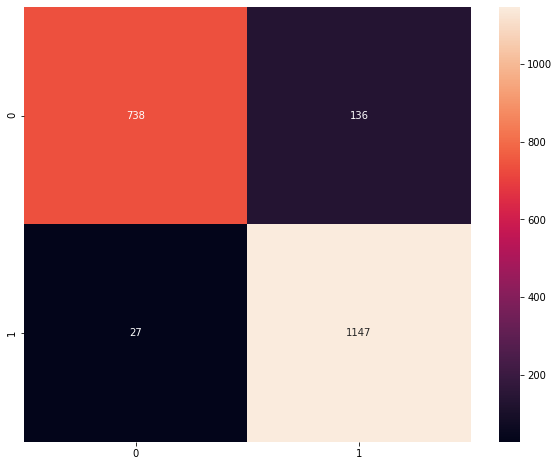
\includegraphics[width=0.5\linewidth]{figuras/quest10_confusaoSVM.png}
    \caption{Matriz de confusão no conjunto de dados de teste para o SVM.}
    \label{fig:quest10_confusaoSVM}
\end{figure}
\FloatBarrier


\thispagestyle{empty}

\newpage
\pagenumbering{arabic}
% % % % % % % % % % % % % % % % % % % % % % % % % % %


\newpage


%\bibliographystyle{abntex2-alf}
%\addcontentsline{toc}{section}{Bibliografia}
%\bibliography{bibliography.bib}


\bibliographystyle{unsrt}
\bibliography{bibliography}
%\noindent AGUIRRE, L. A. Introdução à Identificação de Sistemas, Técnicas Lineares e Não lineares Aplicadas a Sistemas Reais. Belo Horizonte, Brasil, EDUFMG. 2004.\\


\newpage


\end{document}



